% Options for packages loaded elsewhere
\PassOptionsToPackage{unicode}{hyperref}
\PassOptionsToPackage{hyphens}{url}
%
\documentclass[
  russian,
  ignorenonframetext,
]{beamer}
\usepackage{pgfpages}
\setbeamertemplate{caption}[numbered]
\setbeamertemplate{caption label separator}{: }
\setbeamercolor{caption name}{fg=normal text.fg}
\beamertemplatenavigationsymbolsempty
% Prevent slide breaks in the middle of a paragraph
\widowpenalties 1 10000
\raggedbottom
\setbeamertemplate{part page}{
  \centering
  \begin{beamercolorbox}[sep=16pt,center]{part title}
    \usebeamerfont{part title}\insertpart\par
  \end{beamercolorbox}
}
\setbeamertemplate{section page}{
  \centering
  \begin{beamercolorbox}[sep=12pt,center]{part title}
    \usebeamerfont{section title}\insertsection\par
  \end{beamercolorbox}
}
\setbeamertemplate{subsection page}{
  \centering
  \begin{beamercolorbox}[sep=8pt,center]{part title}
    \usebeamerfont{subsection title}\insertsubsection\par
  \end{beamercolorbox}
}
\AtBeginPart{
  \frame{\partpage}
}
\AtBeginSection{
  \ifbibliography
  \else
    \frame{\sectionpage}
  \fi
}
\AtBeginSubsection{
  \frame{\subsectionpage}
}
\usepackage{lmodern}
\usepackage{amssymb,amsmath}
\usepackage{ifxetex,ifluatex}
\ifnum 0\ifxetex 1\fi\ifluatex 1\fi=0 % if pdftex
  \usepackage[T1]{fontenc}
  \usepackage[utf8]{inputenc}
  \usepackage{textcomp} % provide euro and other symbols
\else % if luatex or xetex
  \usepackage{unicode-math}
  \defaultfontfeatures{Scale=MatchLowercase}
  \defaultfontfeatures[\rmfamily]{Ligatures=TeX,Scale=1}
\fi
\usetheme[]{metropolis}
% Use upquote if available, for straight quotes in verbatim environments
\IfFileExists{upquote.sty}{\usepackage{upquote}}{}
\IfFileExists{microtype.sty}{% use microtype if available
  \usepackage[]{microtype}
  \UseMicrotypeSet[protrusion]{basicmath} % disable protrusion for tt fonts
}{}
\makeatletter
\@ifundefined{KOMAClassName}{% if non-KOMA class
  \IfFileExists{parskip.sty}{%
    \usepackage{parskip}
  }{% else
    \setlength{\parindent}{0pt}
    \setlength{\parskip}{6pt plus 2pt minus 1pt}}
}{% if KOMA class
  \KOMAoptions{parskip=half}}
\makeatother
\usepackage{xcolor}
\IfFileExists{xurl.sty}{\usepackage{xurl}}{} % add URL line breaks if available
\IfFileExists{bookmark.sty}{\usepackage{bookmark}}{\usepackage{hyperref}}
\hypersetup{
  pdftitle={Разработка системы обнаружения замаскированных лиц и потенциально опасных персон},
  pdfauthor={Зорин Арсений Геннадьевич},
  pdflang={ru-RU,en-US},
  hidelinks,
  pdfcreator={LaTeX via pandoc}}
\urlstyle{same} % disable monospaced font for URLs
\newif\ifbibliography
\usepackage{graphicx,grffile}
\makeatletter
\def\maxwidth{\ifdim\Gin@nat@width>\linewidth\linewidth\else\Gin@nat@width\fi}
\def\maxheight{\ifdim\Gin@nat@height>\textheight\textheight\else\Gin@nat@height\fi}
\makeatother
% Scale images if necessary, so that they will not overflow the page
% margins by default, and it is still possible to overwrite the defaults
% using explicit options in \includegraphics[width, height, ...]{}
\setkeys{Gin}{width=\maxwidth,height=\maxheight,keepaspectratio}
% Set default figure placement to htbp
\makeatletter
\def\fps@figure{htbp}
\makeatother
\setlength{\emergencystretch}{3em} % prevent overfull lines
\providecommand{\tightlist}{%
  \setlength{\itemsep}{0pt}\setlength{\parskip}{0pt}}
\setcounter{secnumdepth}{-\maxdimen} % remove section numbering
\renewcommand{\caption}[1]{}
\setsansfont[BoldFont={Fira Sans}, Scale=1.20]{Fira Sans}
\setmonofont[Scale=0.95]{Fira Mono}
\metroset{outer/numbering=fraction}
\metroset{titleformat=regular}
\graphicspath{{figs/}}
\ifxetex
  % Load polyglossia as late as possible: uses bidi with RTL langages (e.g. Hebrew, Arabic)
  \usepackage{polyglossia}
  \setmainlanguage[]{}
\else
  \usepackage[shorthands=off,main=russian]{babel}
\fi

\title{Разработка системы обнаружения замаскированных лиц и потенциально
опасных персон}
\author{Зорин Арсений Геннадьевич}
\date{}

\begin{document}
\frame{\titlepage}

\begin{frame}

\begin{block}{Описание проблемы}

\begin{itemize}
\item
  Задержка реагирования (перефразировать)
\item
  Сложно за всем уследить (перефарзировать)
\item
\end{itemize}

\end{block}

\begin{block}{Примеры успешного внедрения машинного обучения}

\begin{block}{Система фиксации нарушений ПДД по видеоизображению}

\end{block}

\begin{block}{Система отслеживания нарушений правил безопасности с
помощью видеоаналитики}

\end{block}

\begin{block}{Автоматическое обнаружение видимых дефектов на выпускаемой
продукции}

\end{block}

\begin{block}{Интеллектуальное управление дорожным движением}

\note{\begin{itemize}
\tightlist
\item
  Ольвия, ООО ``Технологии распознавания''
\item
  Центр2М
\item
  Do not know
\item
  axxonsoft
\end{itemize}}

\end{block}

\end{block}

\begin{block}{Имеющиеся решения}

\begin{block}{Подходы}

\begin{itemize}
\tightlist
\item
  Предсказание ключевых точек
\item
  Поиск Haar-подобных характеристик
\item
  HOG + Adaboost классификатор
\end{itemize}

\end{block}

\begin{block}{}

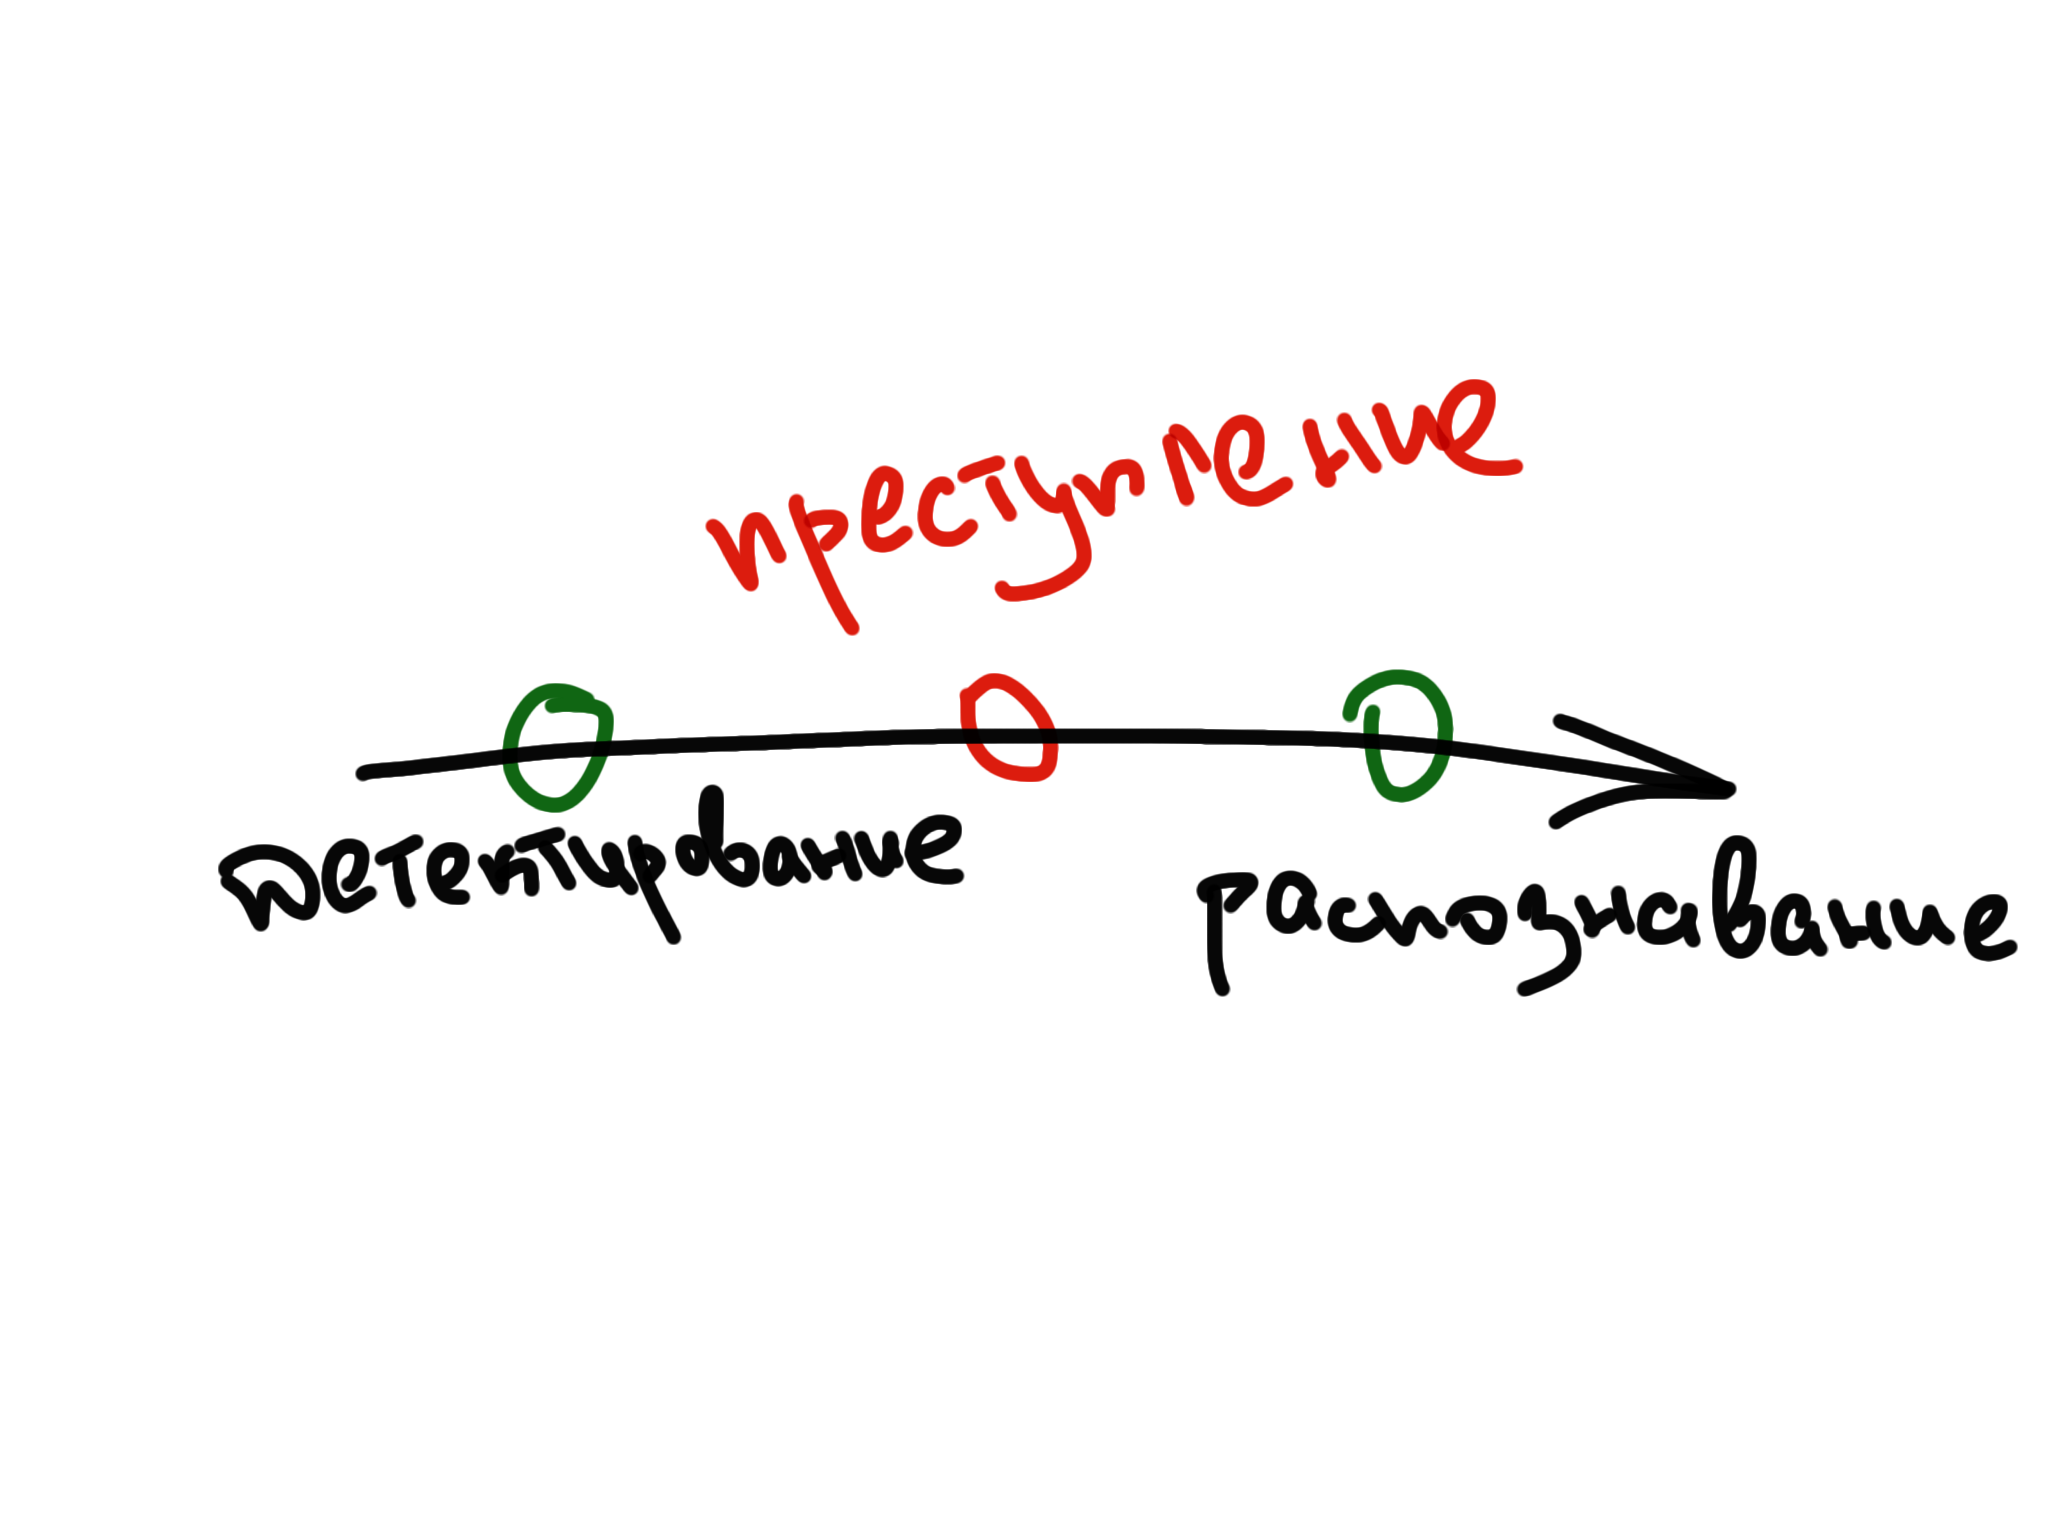
\includegraphics{pics/timeline.png}

\end{block}

\begin{block}{}

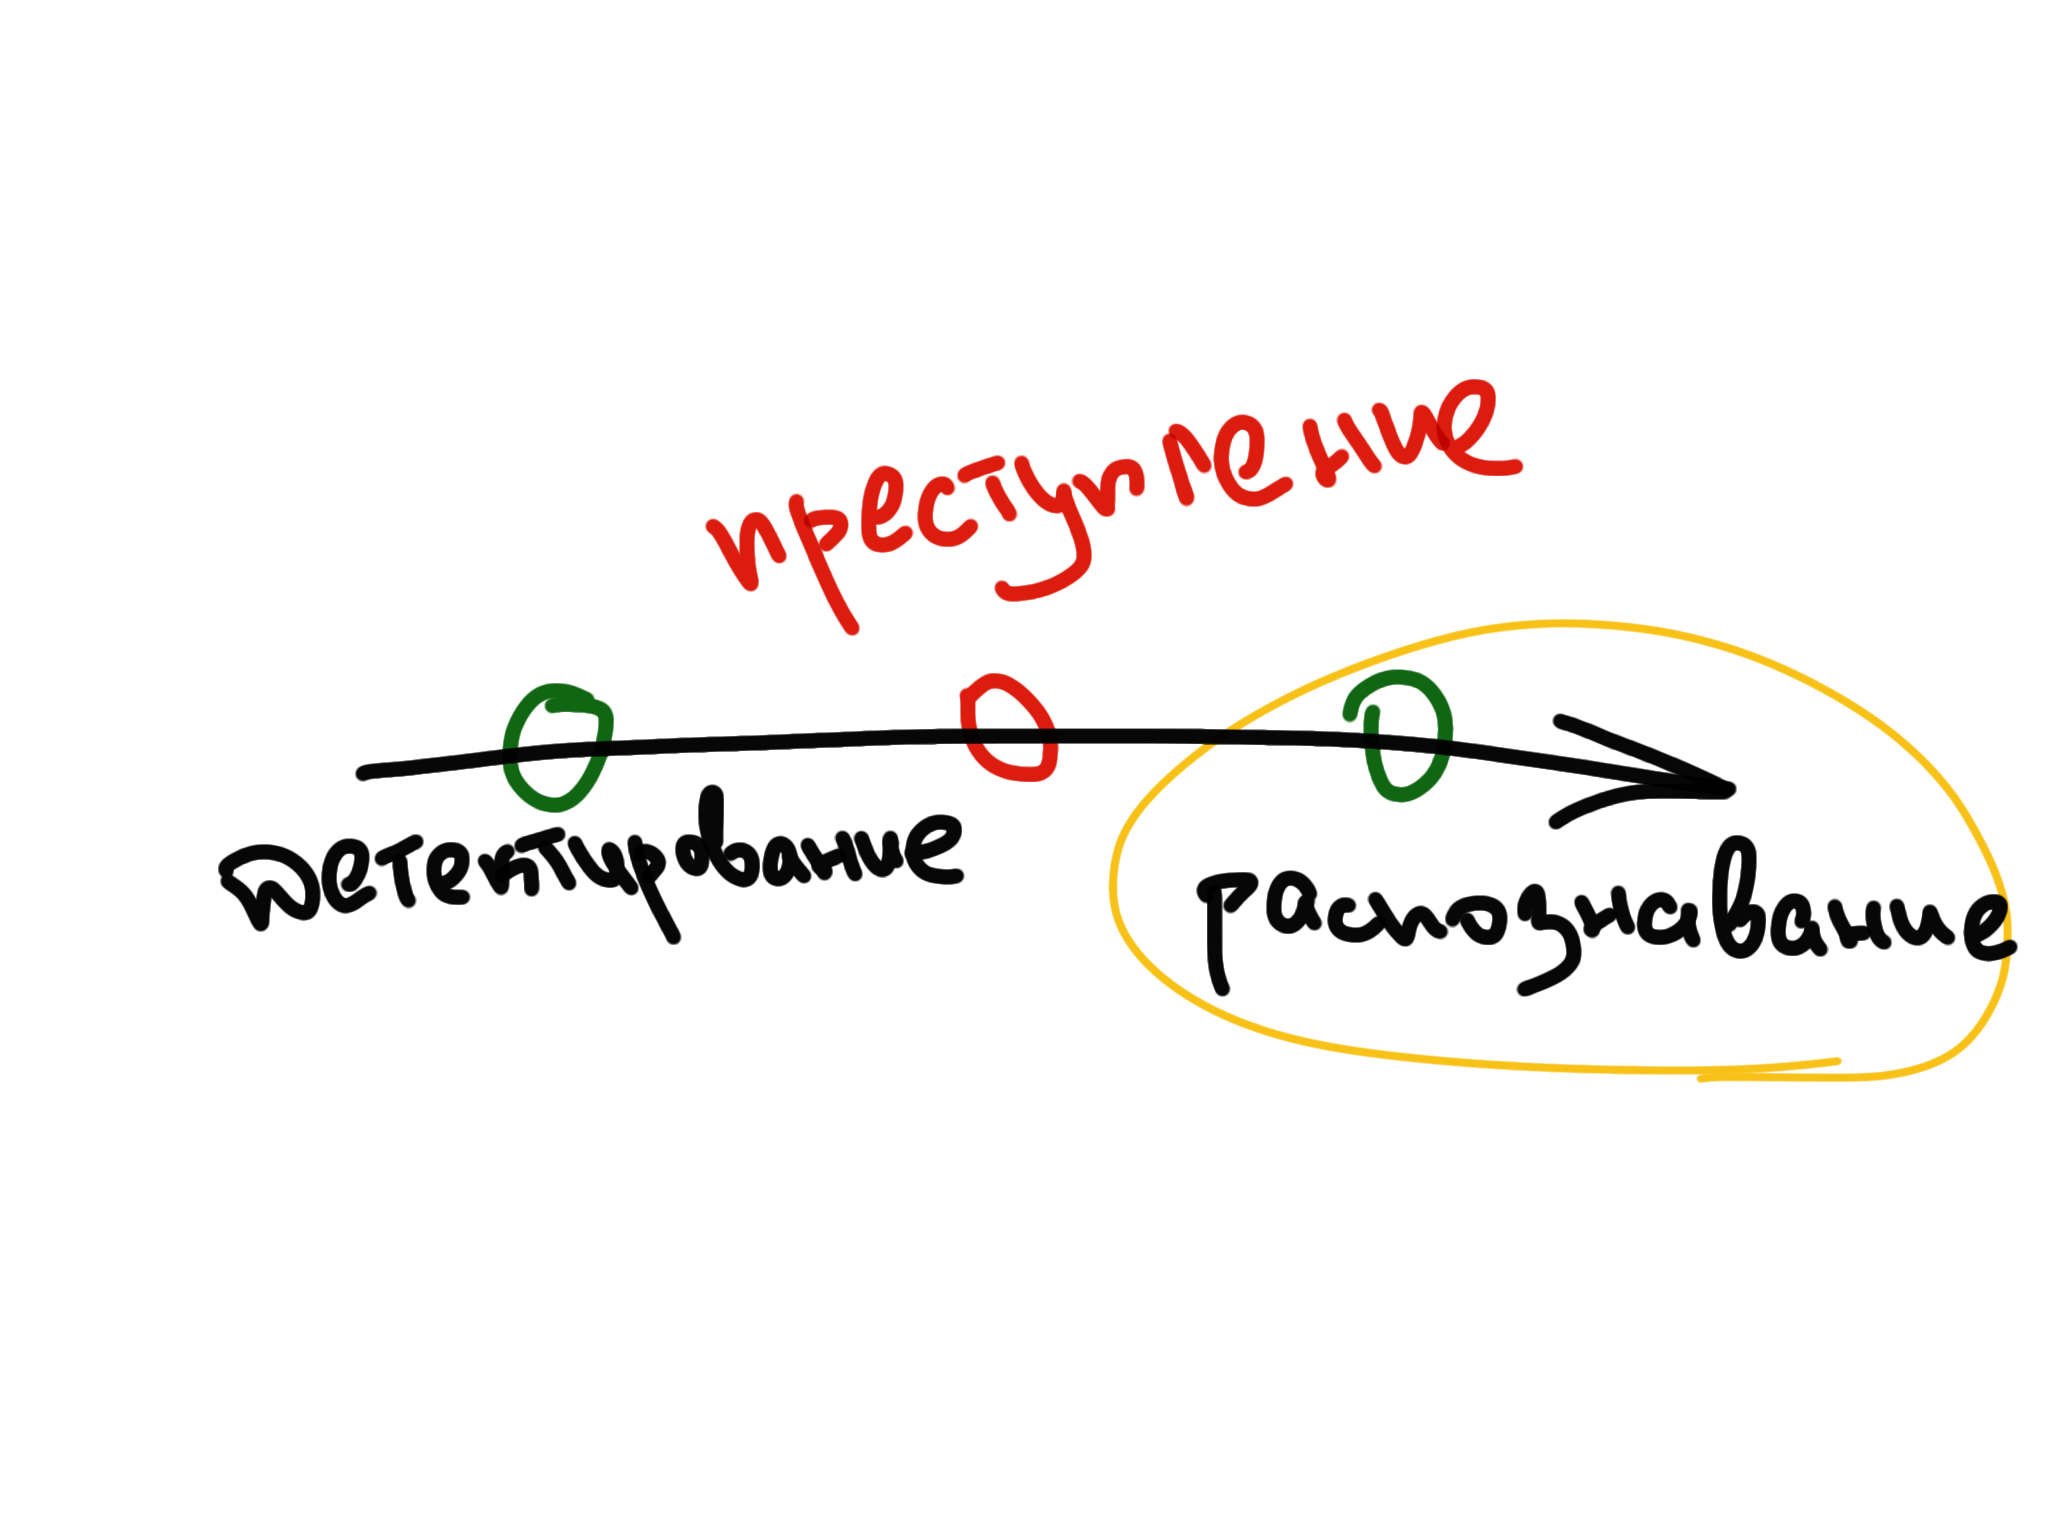
\includegraphics{pics/recogn.png}

\end{block}

\begin{block}{}

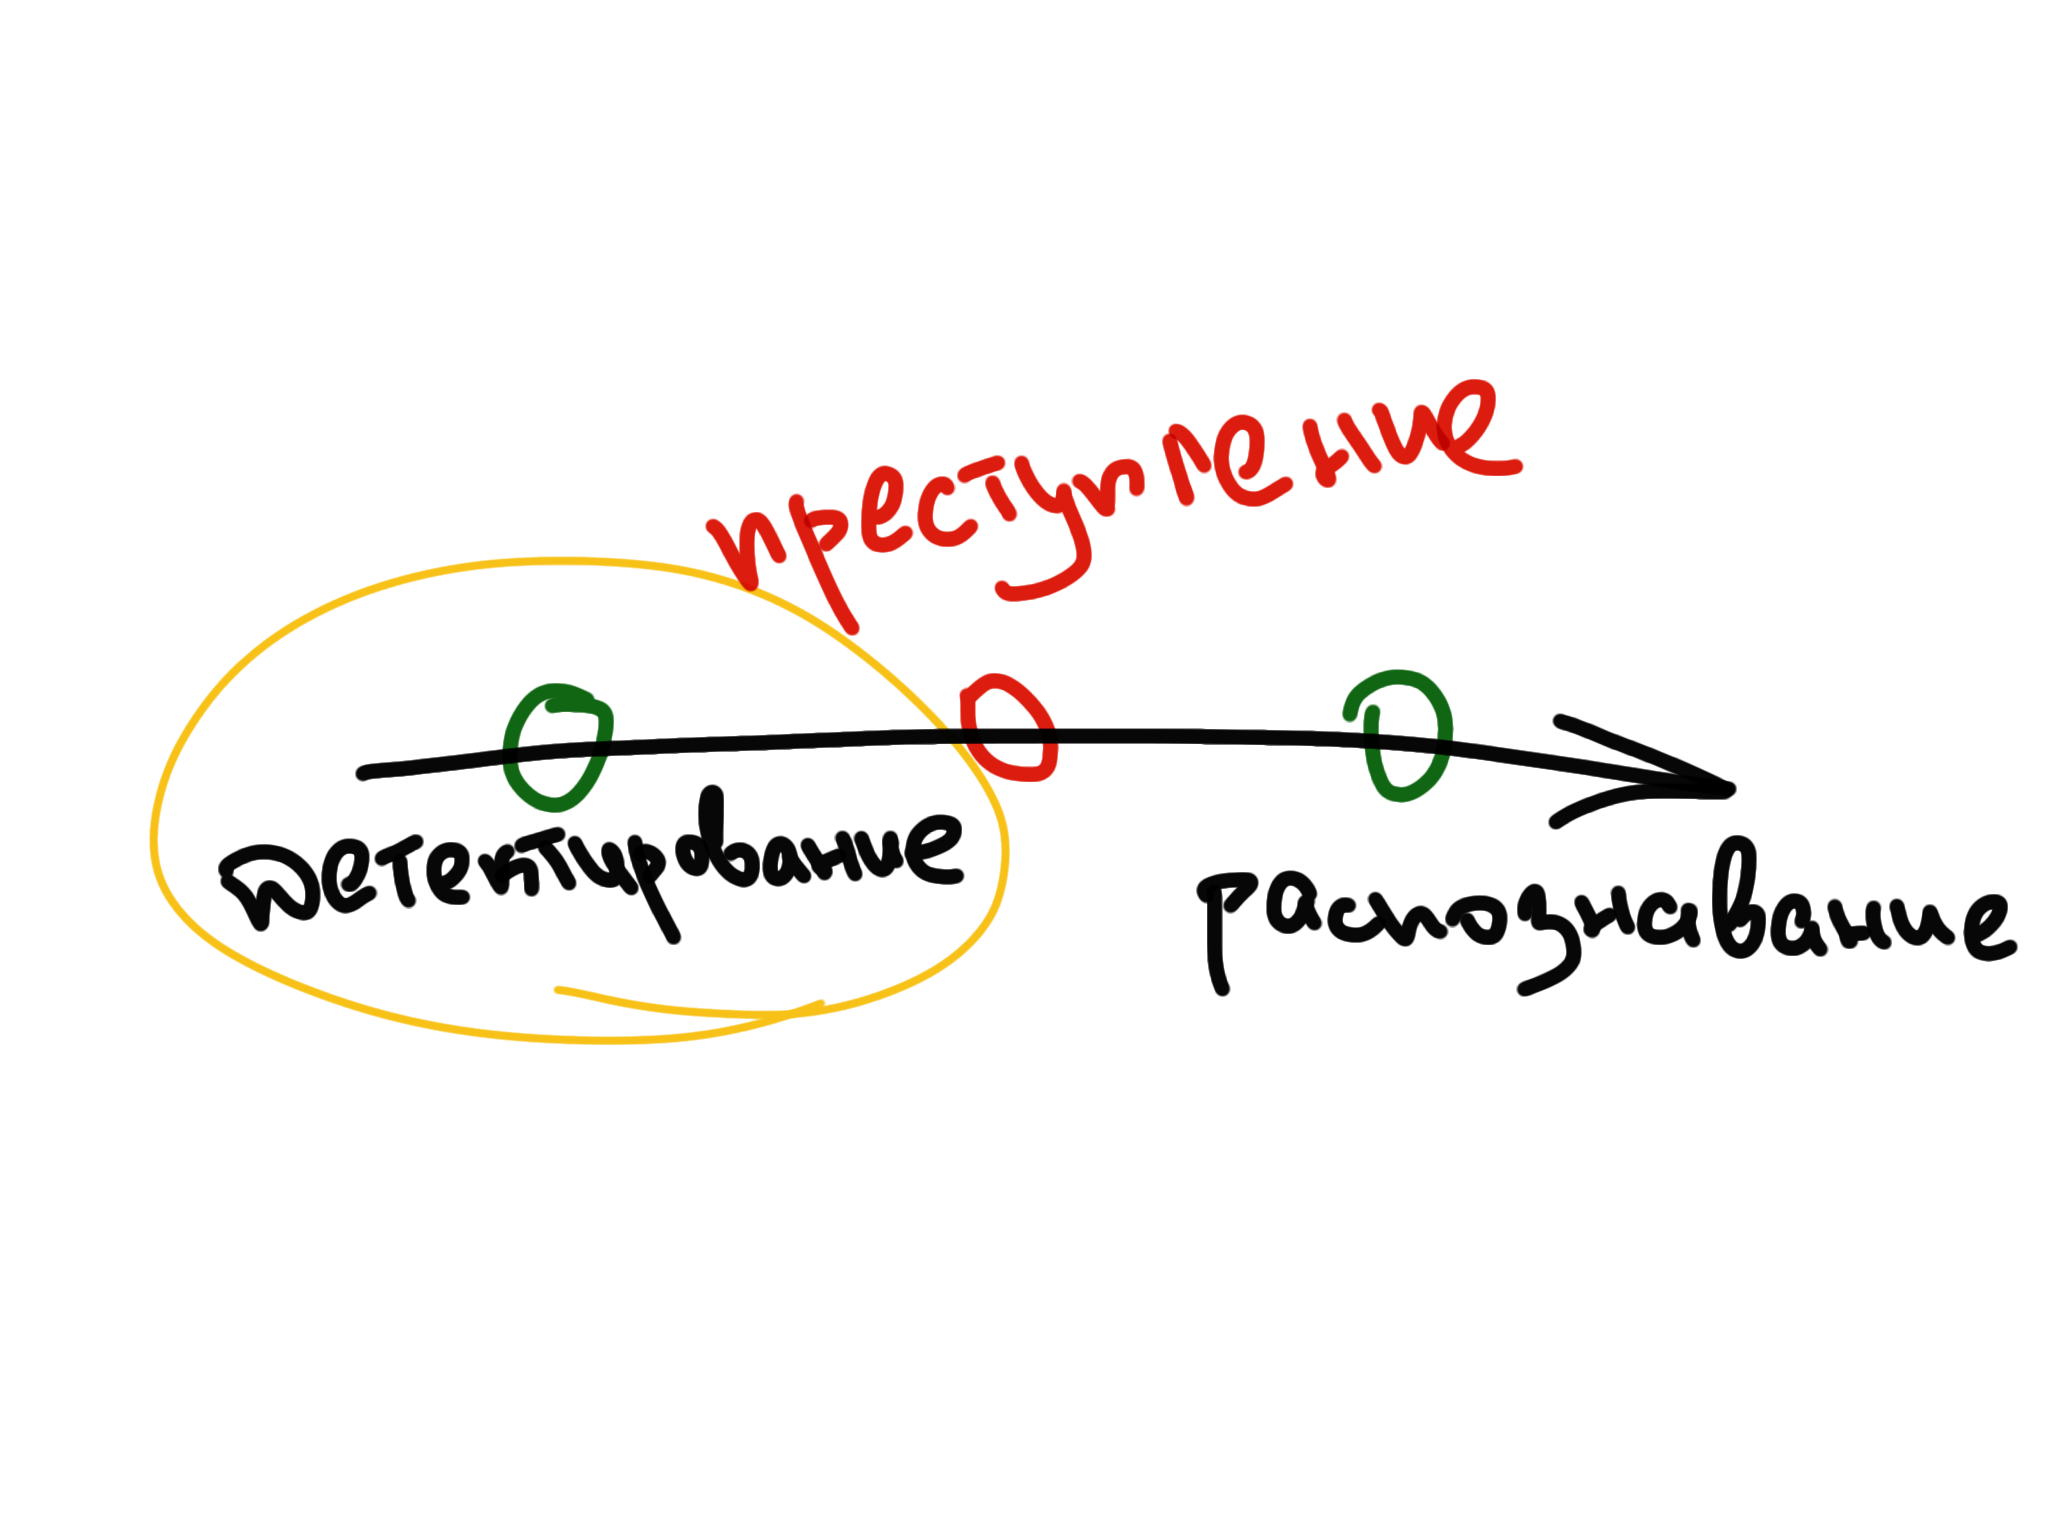
\includegraphics{pics/detection.png}

\end{block}

\end{block}

\begin{block}{Разрабатываемый подход}

\begin{block}{Принцип действия}

\begin{itemize}
\tightlist
\item
  Поиск лица
\item
  Поиск частей лица
\item
  Вывод о состоянии лица (перефразировать. Открытое/Закрытое)
\end{itemize}

\end{block}

\begin{block}{Для поиска лица и частей лица используются сверточные
нейронные сети}

\end{block}

\begin{block}{Вывод о закрытости лица основывается на найденных частях
лица}

\end{block}

\end{block}

\begin{block}{Результаты работы}

\begin{block}{}

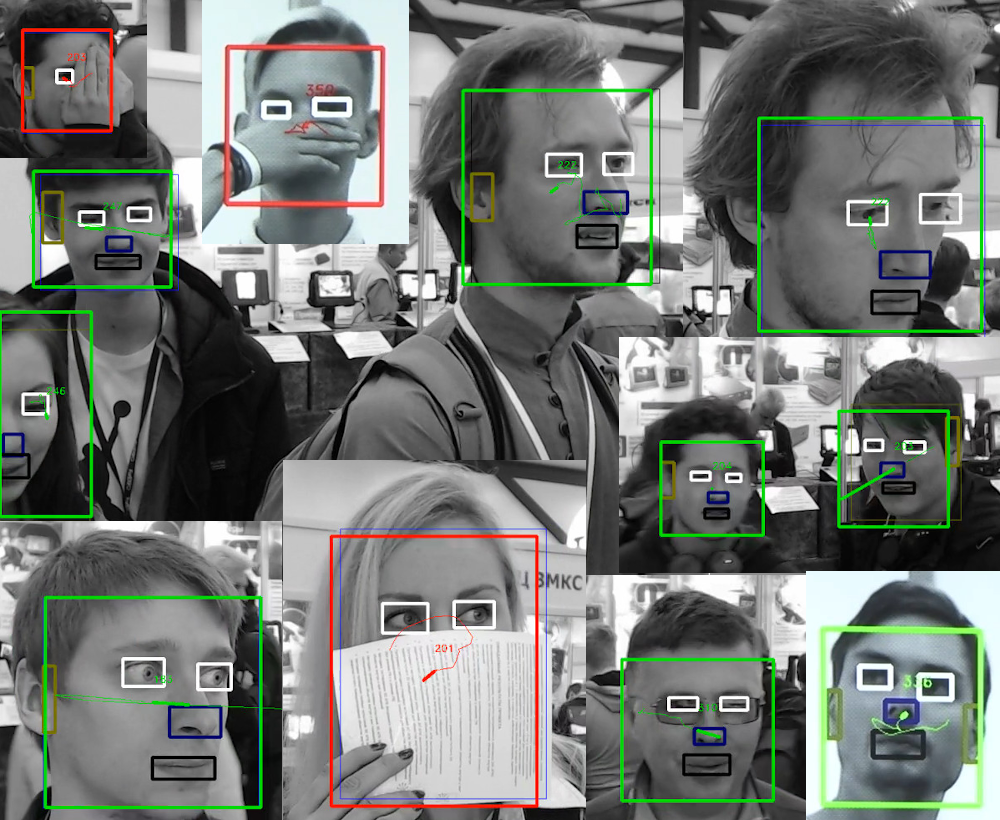
\includegraphics{pics/results.png}

\end{block}

\begin{block}{}

\includegraphics{pics/giphy.gif}

\end{block}

\begin{block}{}

\begin{itemize}
\tightlist
\item
  Точность 83.42\%
\item
  Ресурсоэффективный алгоритм
\item
  Запущен на тестовом стенде
\end{itemize}

\end{block}

\end{block}

\begin{block}{Недостатки метода}

\begin{block}{Закрытое лицо не всегда преступное}

\end{block}

\begin{block}{Результат детектирования зависит от размеров лица}

\end{block}

\begin{block}{}

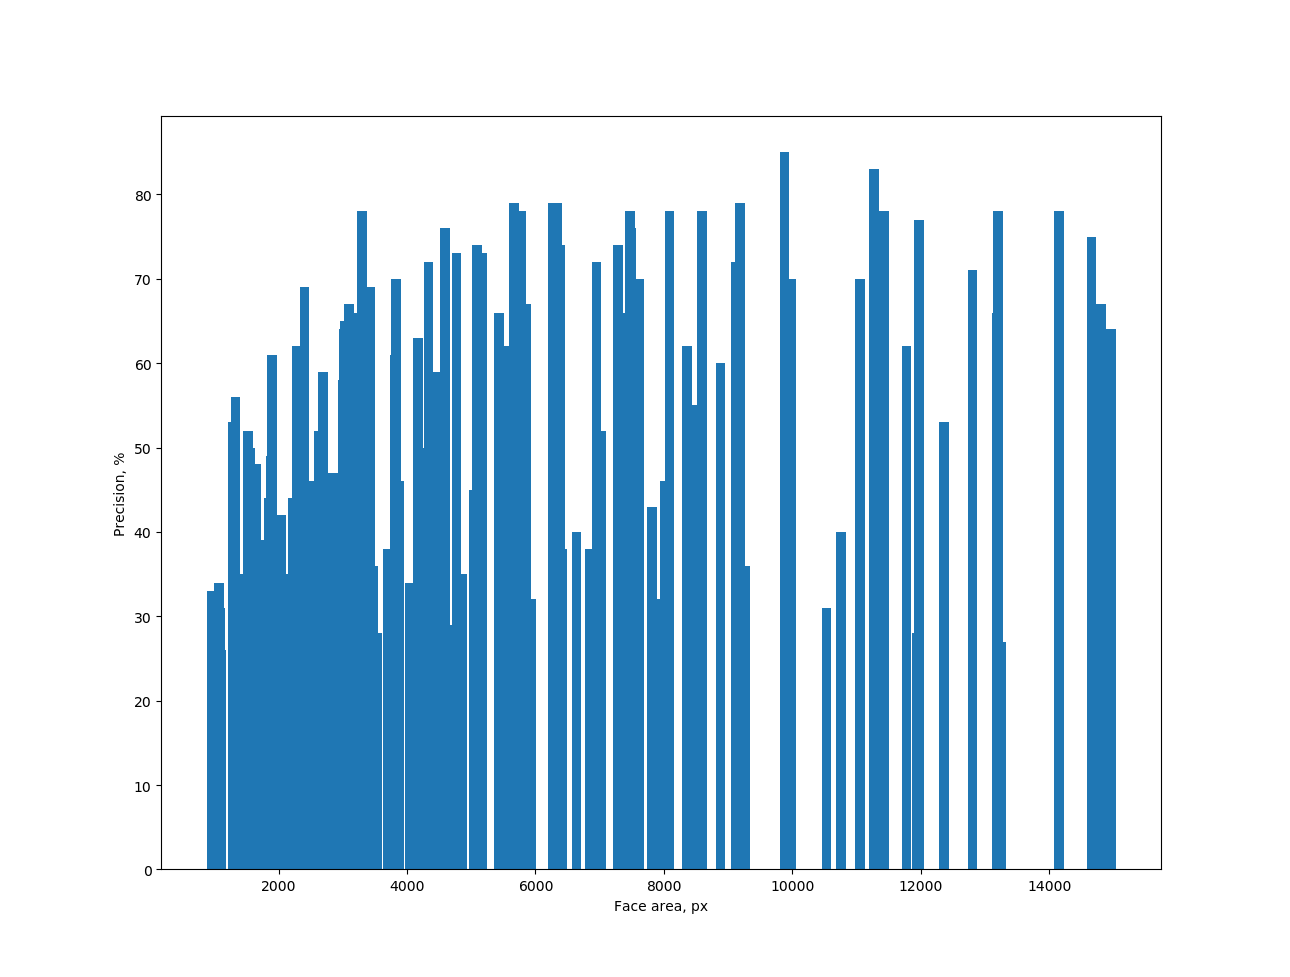
\includegraphics{pics/graph.png}

\end{block}

\end{block}

\begin{block}{Поведенческая модель}

\begin{itemize}
\tightlist
\item
  Что это такое
\item
  Как это
\item
  Что необходимо
\end{itemize}

\end{block}

\begin{block}{Возможные области применения}

\begin{itemize}
\tightlist
\item
  Отделения банков
\item
  Транспортные хабы
\item
  Общедоступные гос. учреждения
\item
  Стадионы
\item
  Места проведения массовых мероприятий
\end{itemize}

\end{block}

\begin{block}{План действий}

\begin{block}{}

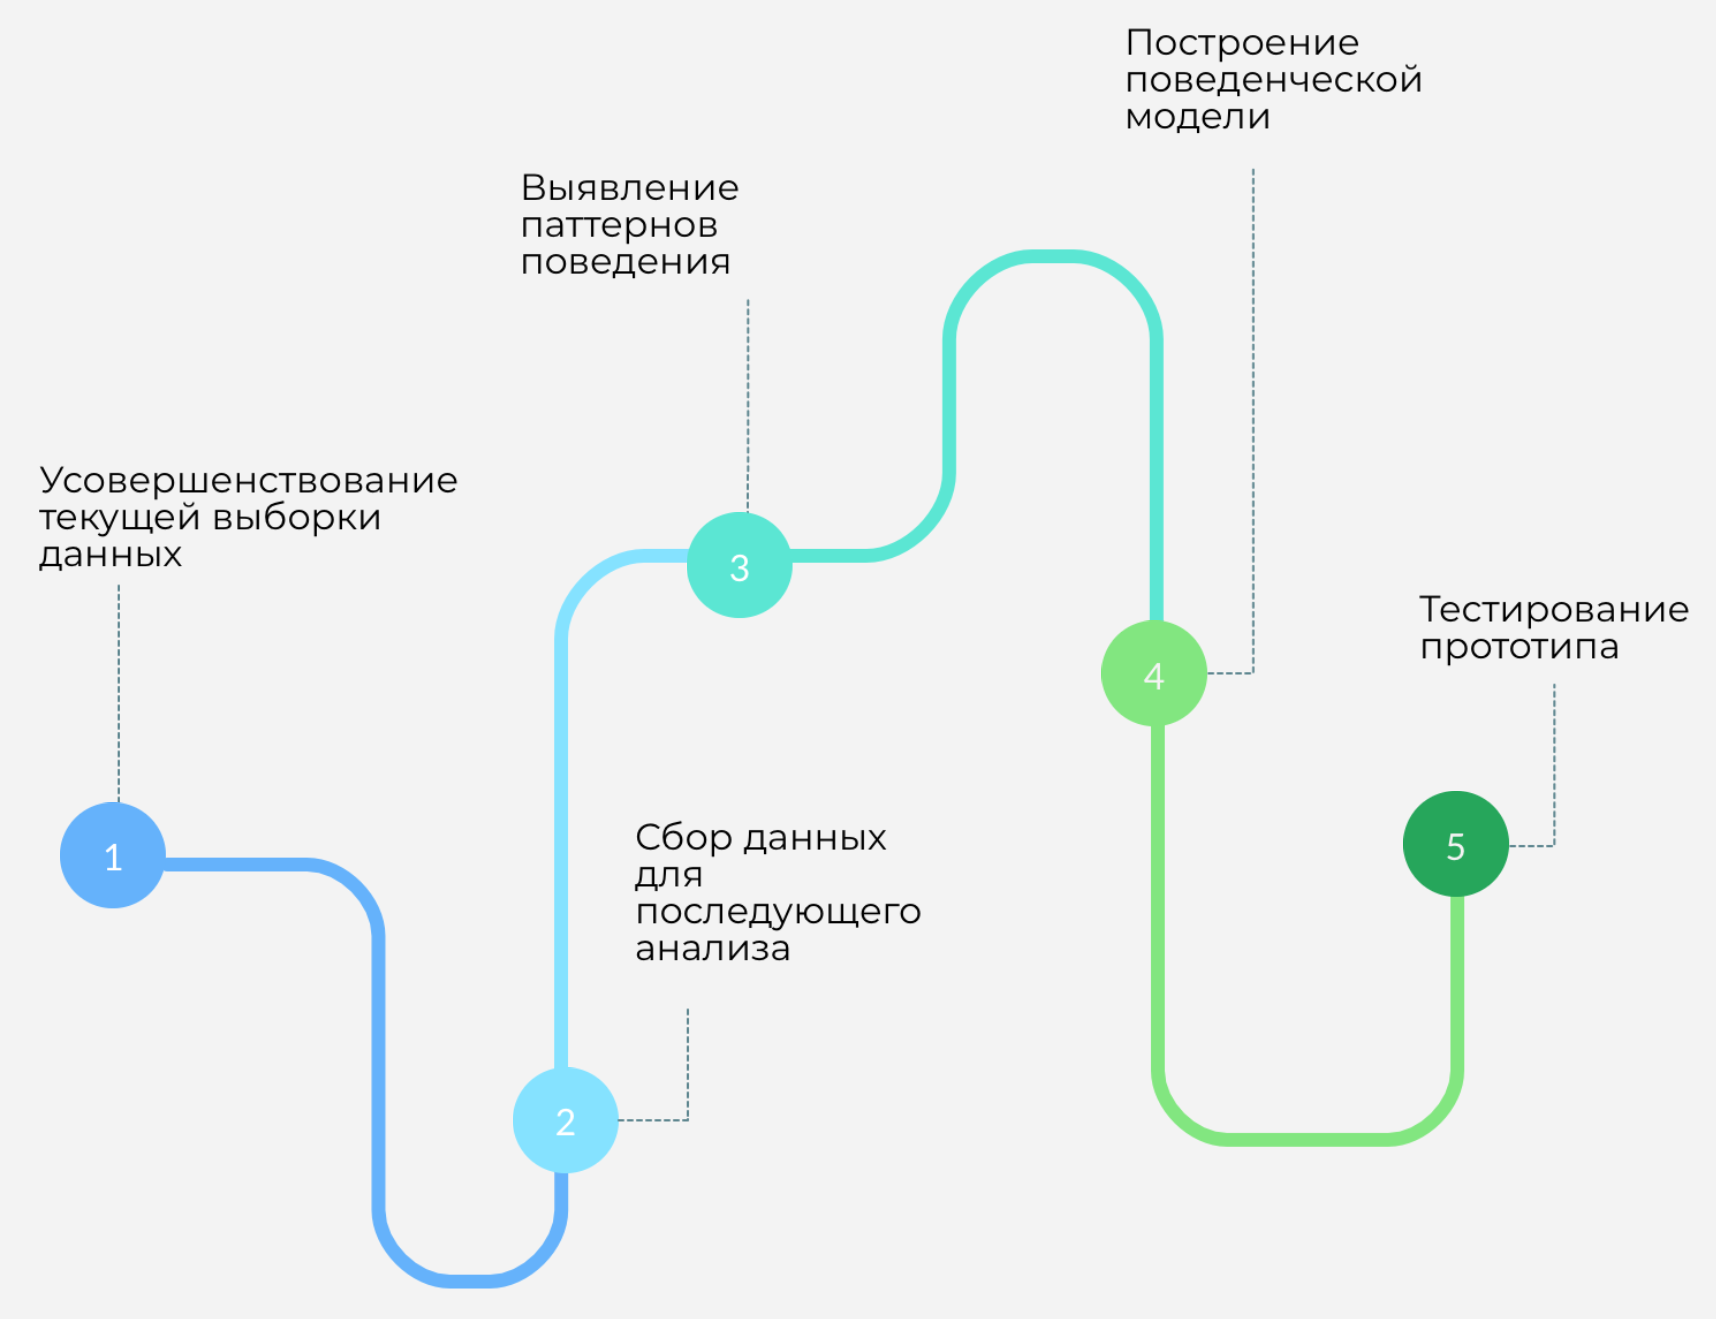
\includegraphics{pics/roadmap.png}

\end{block}

\end{block}

\end{frame}

\begin{frame}{}
\protect\hypertarget{section-8}{}

\begin{itemize}
\tightlist
\item
  E-mail: arseny.zorin@spbpu.com
\item
  GitHub: https://github.com/ArsenyZorin
\item
  GitLab: https://gitlab.com/ArsenyZorin
\end{itemize}

\end{frame}

\end{document}
